% Standardinkluderingsfil
\input{standard}

\ifpdf
  \DeclareGraphicsExtensions{.pdf, .jpg, .tif, .png}
  \pdfinfo{            
    /Title  (Use-case model)
    /Author (PUM-grupp 1)
  }
\else
  \DeclareGraphicsExtensions{.eps, .jpg}
\fi

\title{Distribuerad wiki \\ Use-case model \\ Version 1.1}
\author{PUM-grupp 1}
\date{\today}

\begin{document}

\maketitle\thispagestyle{empty}
\newpage

{\centering \Large{Dokumenthistorik\\}}

\vspace{10pt}
\begin{tabularx}{\textwidth}{ |l|l|X|l|l| }
  \hline
    \textbf{version} & \textbf{datum} & \textbf{utförda ändringar} & \textbf{utförda av} & \textbf{granskad} \\
	\hline 
  1.0 & 2009-02-12 &  Första versionen klar för inlämning  & Alla & Alla   \\
  \hline 1.1 & 2009-03-09 & Reviderad version & Martin & INGEN\\
  \hline
\end{tabularx}

\newpage
\setcounter{tocdepth}{2}
\tableofcontents
\newpage

\section{Inledning}
För att enklare förstå de olika användarfallen vi identifierat och skapa en överblick över dem har vi gjort en användarfalls model där vi grafisk visar hur användare och system hänger ihop.
\section{Överblick}
%Skapa en överblick för systemet, dvs beskriv vad systemet gör och vad desss mål är.
Systemet i fråga är ett distribuerat versionshanteringssystem. Meningen med detta system är att man på ett enkelt sätt ska kunna hantera dokument i en wiki-miljö samtidigt som man inte ens behöver vara uppkopplad. När användaren sedan kopplar upp sig mot internet kan denne synkronisera sina ändringar med andra användares ändringar.
\section{Användarfallsdiagram}
 \begin{figure}[H] %  figure placement: here, top, bottom, or page
  \centering
  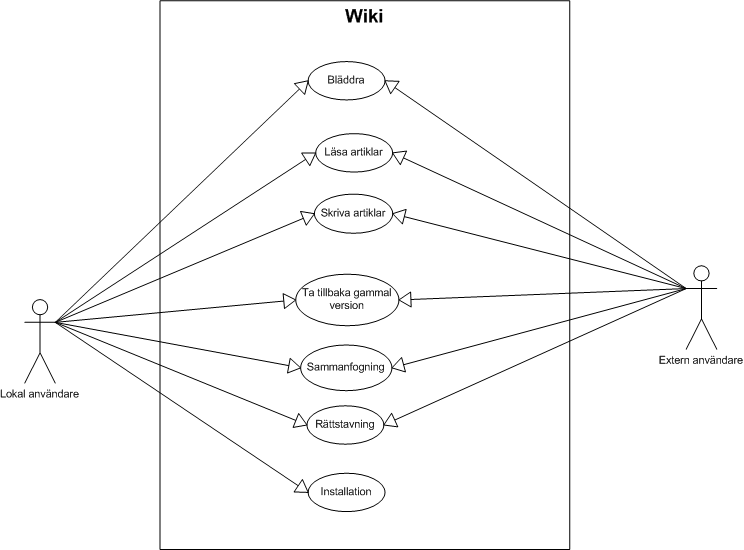
\includegraphics[scale=0.50]{Use-case-diagram.png}
\end{figure}
%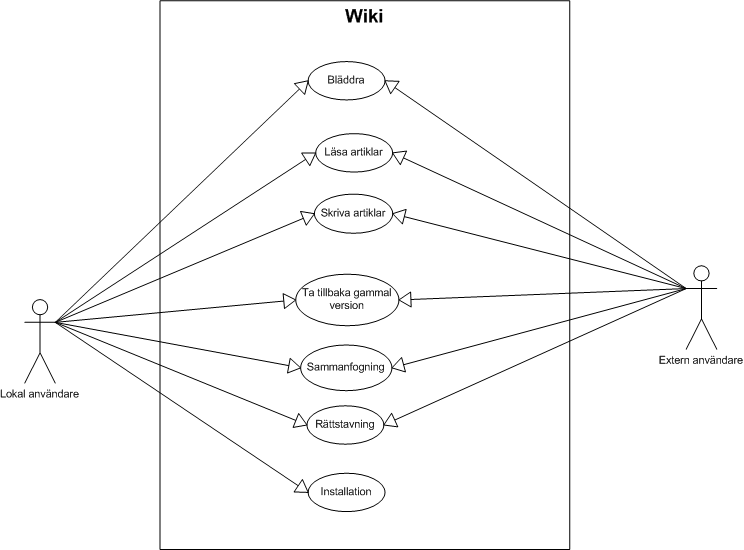
\includegraphics{Use-case-diagram.png}
\section{Aktörer}
%Beskriv alla aktörer som finns med i use-case diagrammet.
\begin{itemize}
	\item Lokal användare
	\\Denna aktör representerar en normal användare som sitter vid sin dator och ej är uppkopplad mot internet.
	\item Extern användare
	\\Denna aktör representerar en användare som sitter uppkopplad mot systemet och internet.
\end{itemize}
\newpage
\section{Användarfall}
%Rada upp de olika use-cases som finns.
\subsection{Installation}
Detta användarfall beskriver hur man installerar systemet.
\subsection{Bläddra}
Detta användarfall beskriver hur man bläddrar bland dokument.
\subsection{Läsa artiklar}
Detta användarfall beskriver hur man läser sina egna eller andra användares artiklar.
\subsection{Skriva en artikel}
Detta användarfall beskriver hur man skriver en artikel.
\subsection{Ta tillbaka gammal version}
Detta användarfall beskriver hur man tar tillbaka en gammal version av en fil.
\subsection{Sammanslagning}
Detta användarfall beskriver hur man sammanfogar två eller flera filer med varandra.
\subsection{Rättstavning}
Detta användarfall beskriver hur man kan använda rättstavningskontrollen.
\end{document}
